\documentclass{standalone}
\usepackage{tikz}
\usetikzlibrary{patterns, positioning}

\begin{document}
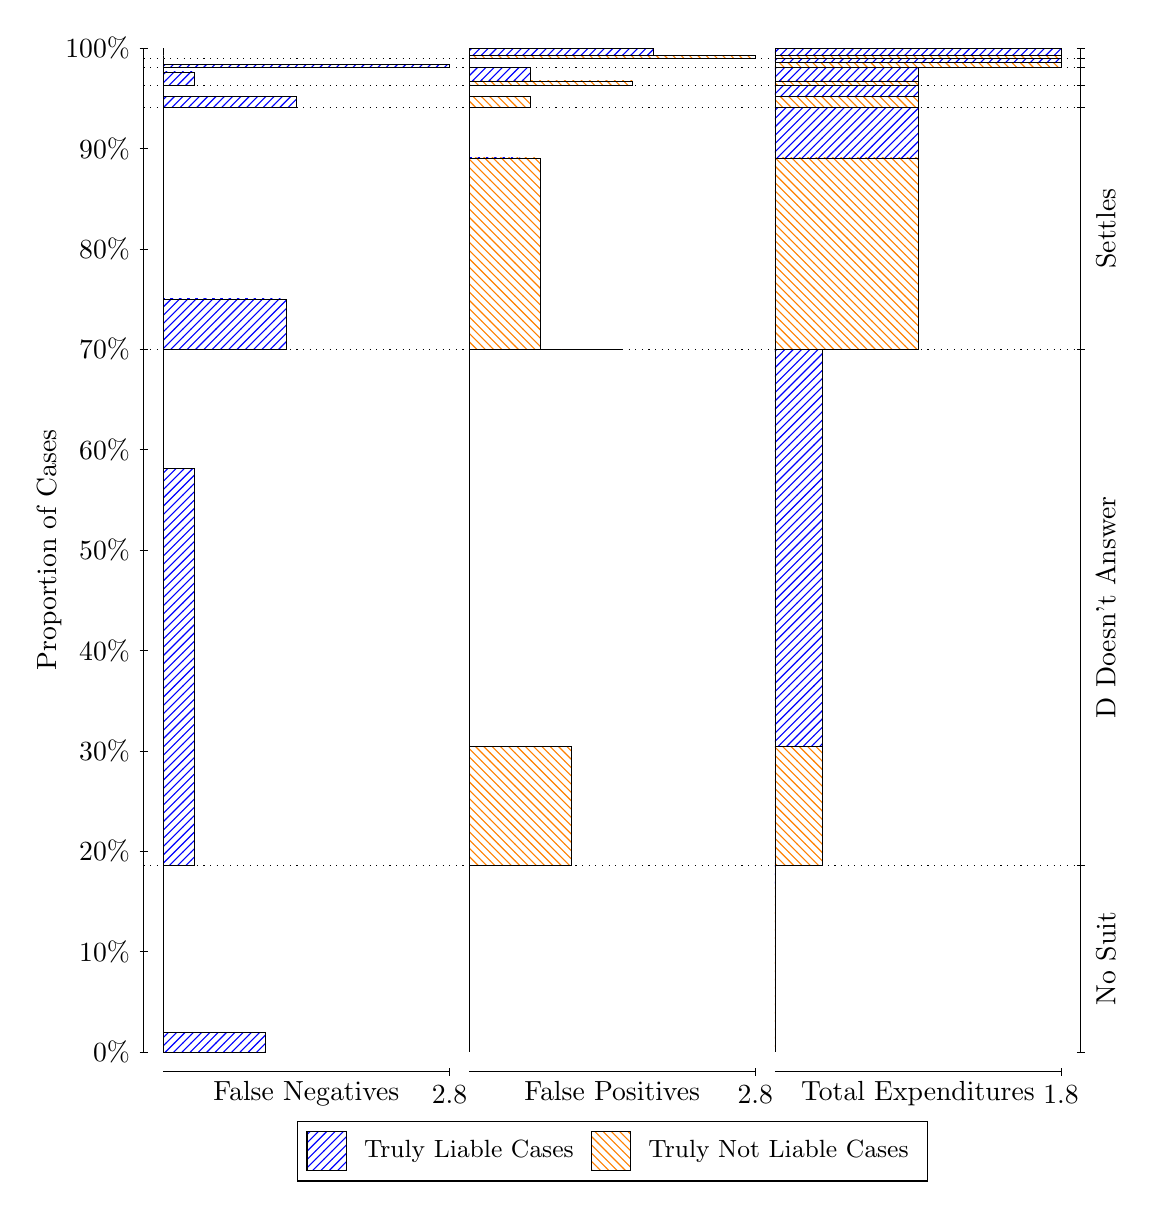
\begin{tikzpicture}
\draw[black, very thin] (1.5,1.75) -- (1.5,14.5);
\node[rotate=90, anchor=center] at (0.3, 8.125) {Proportion of Cases};
\draw[black, very thin] (1.45,1.75) -- (1.55,1.75);
\node[anchor=east] at (1.45, 1.75) {0\%};
\draw[black, very thin] (1.45,3.025) -- (1.55,3.025);
\node[anchor=east] at (1.45, 3.025) {10\%};
\draw[black, very thin] (1.45,4.3) -- (1.55,4.3);
\node[anchor=east] at (1.45, 4.3) {20\%};
\draw[black, very thin] (1.45,5.575) -- (1.55,5.575);
\node[anchor=east] at (1.45, 5.575) {30\%};
\draw[black, very thin] (1.45,6.85) -- (1.55,6.85);
\node[anchor=east] at (1.45, 6.85) {40\%};
\draw[black, very thin] (1.45,8.125) -- (1.55,8.125);
\node[anchor=east] at (1.45, 8.125) {50\%};
\draw[black, very thin] (1.45,9.4) -- (1.55,9.4);
\node[anchor=east] at (1.45, 9.4) {60\%};
\draw[black, very thin] (1.45,10.675) -- (1.55,10.675);
\node[anchor=east] at (1.45, 10.675) {70\%};
\draw[black, very thin] (1.45,11.95) -- (1.55,11.95);
\node[anchor=east] at (1.45, 11.95) {80\%};
\draw[black, very thin] (1.45,13.225) -- (1.55,13.225);
\node[anchor=east] at (1.45, 13.225) {90\%};
\draw[black, very thin] (1.45,14.5) -- (1.55,14.5);
\node[anchor=east] at (1.45, 14.5) {100\%};

\draw[black, very thin] (13.4,1.75) -- (13.4,14.5);
\draw[black, very thin] (13.35,1.75) -- (13.45,1.75);
\node[anchor=west] at (13.35, 1.75) {};
\draw[black, very thin] (13.35,4.1224) -- (13.45,4.1224);
\node[anchor=west] at (13.35, 4.1224) {};
\draw[black, very thin] (13.35,10.673) -- (13.45,10.673);
\node[anchor=west] at (13.35, 10.673) {};
\draw[black, very thin] (13.35,13.745) -- (13.45,13.745);
\node[anchor=west] at (13.35, 13.745) {};
\draw[black, very thin] (13.35,14.029) -- (13.45,14.029);
\node[anchor=west] at (13.35, 14.029) {};
\draw[black, very thin] (13.35,14.251) -- (13.45,14.251);
\node[anchor=west] at (13.35, 14.251) {};
\draw[black, very thin] (13.35,14.365) -- (13.45,14.365);
\node[anchor=west] at (13.35, 14.365) {};
\draw[black, very thin] (13.35,14.5) -- (13.45,14.5);
\node[anchor=west] at (13.35, 14.5) {};

\draw[black, very thin, pattern color=blue, pattern=north east lines] (1.75,1.75) rectangle (3.0476,1.9996);
\draw[black, very thin, pattern color=orange, pattern=north west lines] (1.75,1.9996) rectangle (1.75,4.1224);
\draw[black, very thin, pattern color=blue, pattern=north east lines] (1.75,4.1224) rectangle (2.1393,9.1638);
\draw[black, very thin, pattern color=orange, pattern=north west lines] (1.75,9.1638) rectangle (1.75,10.673);
\draw[black, very thin, pattern color=blue, pattern=north east lines] (1.75,10.673) rectangle (3.3071,11.313);
\draw[black, very thin, pattern color=blue, pattern=north east lines] (1.75,11.313) rectangle (3.1774,11.313);
\draw[black, very thin, pattern color=blue, pattern=north east lines] (1.75,11.313) rectangle (3.0476,11.313);
\draw[black, very thin, pattern color=blue, pattern=north east lines] (1.75,11.313) rectangle (2.9179,11.313);
\draw[black, very thin, pattern color=blue, pattern=north east lines] (1.75,11.313) rectangle (2.9179,11.313);
\draw[black, very thin, pattern color=blue, pattern=north east lines] (1.75,11.313) rectangle (2.7881,11.313);
\draw[black, very thin, pattern color=blue, pattern=north east lines] (1.75,11.313) rectangle (2.6583,11.313);
\draw[black, very thin, pattern color=blue, pattern=north east lines] (1.75,11.313) rectangle (2.5286,11.313);
\draw[black, very thin, pattern color=blue, pattern=north east lines] (1.75,11.313) rectangle (2.3988,11.313);
\draw[black, very thin, pattern color=blue, pattern=north east lines] (1.75,11.313) rectangle (2.269,11.313);
\draw[black, very thin, pattern color=orange, pattern=north west lines] (1.75,11.313) rectangle (1.75,13.745);
\draw[black, very thin, pattern color=blue, pattern=north east lines] (1.75,13.745) rectangle (3.4369,13.886);
\draw[black, very thin, pattern color=orange, pattern=north west lines] (1.75,13.886) rectangle (1.75,14.029);
\draw[black, very thin, pattern color=blue, pattern=north east lines] (1.75,14.029) rectangle (2.1393,14.196);
\draw[black, very thin, pattern color=orange, pattern=north west lines] (1.75,14.196) rectangle (1.75,14.251);
\draw[black, very thin, pattern color=blue, pattern=north east lines] (1.75,14.251) rectangle (5.3833,14.295);
\draw[black, very thin, pattern color=orange, pattern=north west lines] (1.75,14.295) rectangle (1.75,14.365);
\draw[black, very thin, pattern color=orange, pattern=north west lines] (1.75,14.365) rectangle (1.75,14.408);
\draw[black, very thin, pattern color=blue, pattern=north east lines] (1.75,14.408) rectangle (1.75,14.5);
\draw[black, very thin, pattern color=orange, pattern=north west lines] (5.6333,1.75) rectangle (5.6333,3.8728);
\draw[black, very thin, pattern color=blue, pattern=north east lines] (5.6333,3.8728) rectangle (5.6333,4.1224);
\draw[black, very thin, pattern color=orange, pattern=north west lines] (5.6333,4.1224) rectangle (6.931,5.6319);
\draw[black, very thin, pattern color=blue, pattern=north east lines] (5.6333,5.6319) rectangle (5.6333,10.673);
\draw[black, very thin, pattern color=orange, pattern=north west lines] (5.6333,10.673) rectangle (7.5798,10.673);
\draw[black, very thin, pattern color=orange, pattern=north west lines] (5.6333,10.673) rectangle (7.45,10.673);
\draw[black, very thin, pattern color=orange, pattern=north west lines] (5.6333,10.673) rectangle (7.3202,10.673);
\draw[black, very thin, pattern color=orange, pattern=north west lines] (5.6333,10.673) rectangle (7.1905,10.673);
\draw[black, very thin, pattern color=orange, pattern=north west lines] (5.6333,10.673) rectangle (7.0607,10.673);
\draw[black, very thin, pattern color=orange, pattern=north west lines] (5.6333,10.673) rectangle (6.931,10.673);
\draw[black, very thin, pattern color=orange, pattern=north west lines] (5.6333,10.673) rectangle (6.8012,10.673);
\draw[black, very thin, pattern color=orange, pattern=north west lines] (5.6333,10.673) rectangle (6.6714,10.673);
\draw[black, very thin, pattern color=orange, pattern=north west lines] (5.6333,10.673) rectangle (6.5417,13.105);
\draw[black, very thin, pattern color=blue, pattern=north east lines] (5.6333,13.105) rectangle (6.2821,13.105);
\draw[black, very thin, pattern color=blue, pattern=north east lines] (5.6333,13.105) rectangle (6.1524,13.105);
\draw[black, very thin, pattern color=blue, pattern=north east lines] (5.6333,13.105) rectangle (6.0226,13.105);
\draw[black, very thin, pattern color=blue, pattern=north east lines] (5.6333,13.105) rectangle (5.8929,13.105);
\draw[black, very thin, pattern color=blue, pattern=north east lines] (5.6333,13.105) rectangle (5.7631,13.105);
\draw[black, very thin, pattern color=blue, pattern=north east lines] (5.6333,13.105) rectangle (5.6333,13.745);
\draw[black, very thin, pattern color=orange, pattern=north west lines] (5.6333,13.745) rectangle (6.4119,13.888);
\draw[black, very thin, pattern color=blue, pattern=north east lines] (5.6333,13.888) rectangle (5.6333,14.029);
\draw[black, very thin, pattern color=orange, pattern=north west lines] (5.6333,14.029) rectangle (7.7095,14.084);
\draw[black, very thin, pattern color=blue, pattern=north east lines] (5.6333,14.084) rectangle (6.4119,14.251);
\draw[black, very thin, pattern color=orange, pattern=north west lines] (5.6333,14.251) rectangle (5.6333,14.322);
\draw[black, very thin, pattern color=blue, pattern=north east lines] (5.6333,14.322) rectangle (5.6333,14.365);
\draw[black, very thin, pattern color=orange, pattern=north west lines] (5.6333,14.365) rectangle (9.2667,14.408);
\draw[black, very thin, pattern color=blue, pattern=north east lines] (5.6333,14.408) rectangle (7.969,14.5);
\draw[black, very thin, pattern color=orange, pattern=north west lines] (9.5167,1.75) rectangle (9.5167,3.8728);
\draw[black, very thin, pattern color=blue, pattern=north east lines] (9.5167,3.8728) rectangle (9.5167,4.1224);
\draw[black, very thin, pattern color=orange, pattern=north west lines] (9.5167,4.1224) rectangle (10.122,5.6319);
\draw[black, very thin, pattern color=blue, pattern=north east lines] (9.5167,5.6319) rectangle (10.122,10.673);
\draw[black, very thin, pattern color=orange, pattern=north west lines] (9.5167,10.673) rectangle (11.333,10.673);
\draw[black, very thin, pattern color=blue, pattern=north east lines] (9.5167,10.673) rectangle (11.333,10.673);
\draw[black, very thin, pattern color=orange, pattern=north west lines] (9.5167,10.673) rectangle (11.333,10.673);
\draw[black, very thin, pattern color=blue, pattern=north east lines] (9.5167,10.673) rectangle (11.333,10.673);
\draw[black, very thin, pattern color=orange, pattern=north west lines] (9.5167,10.673) rectangle (11.333,13.105);
\draw[black, very thin, pattern color=blue, pattern=north east lines] (9.5167,13.105) rectangle (11.333,13.745);
\draw[black, very thin, pattern color=orange, pattern=north west lines] (9.5167,13.745) rectangle (11.333,13.888);
\draw[black, very thin, pattern color=blue, pattern=north east lines] (9.5167,13.888) rectangle (11.333,14.029);
\draw[black, very thin, pattern color=orange, pattern=north west lines] (9.5167,14.029) rectangle (11.333,14.084);
\draw[black, very thin, pattern color=blue, pattern=north east lines] (9.5167,14.084) rectangle (11.333,14.251);
\draw[black, very thin, pattern color=orange, pattern=north west lines] (9.5167,14.251) rectangle (13.15,14.322);
\draw[black, very thin, pattern color=blue, pattern=north east lines] (9.5167,14.322) rectangle (13.15,14.365);
\draw[black, very thin, pattern color=orange, pattern=north west lines] (9.5167,14.365) rectangle (13.15,14.408);
\draw[black, very thin, pattern color=blue, pattern=north east lines] (9.5167,14.408) rectangle (13.15,14.5);
\draw[black, dotted] (1.5,4.1224) -- (13.4,4.1224);
\draw[black, dotted] (1.5,10.673) -- (13.4,10.673);
\draw[black, dotted] (1.5,13.745) -- (13.4,13.745);
\draw[black, dotted] (1.5,14.029) -- (13.4,14.029);
\draw[black, dotted] (1.5,14.251) -- (13.4,14.251);
\draw[black, dotted] (1.5,14.365) -- (13.4,14.365);
\draw[black, very thin] (1.75,1.5) -- (5.3833,1.5);
\node[anchor=north] at (3.5667, 1.5) {False Negatives};
\draw[black, very thin] (5.3833,1.45) -- (5.3833,1.55);
\node[anchor=north] at (5.3833, 1.45) {2.8};

\draw[black, very thin] (5.6333,1.5) -- (9.2667,1.5);
\node[anchor=north] at (7.45, 1.5) {False Positives};
\draw[black, very thin] (9.2667,1.45) -- (9.2667,1.55);
\node[anchor=north] at (9.2667, 1.45) {2.8};

\draw[black, very thin] (9.5167,1.5) -- (13.15,1.5);
\node[anchor=north] at (11.333, 1.5) {Total Expenditures};
\draw[black, very thin] (13.15,1.45) -- (13.15,1.55);
\node[anchor=north] at (13.15, 1.45) {1.8};

\node[black, centered, rotate=90] at (13.72, 2.9362) {No Suit};
\node[black, centered, rotate=90] at (13.72, 7.3978) {D Doesn't Answer};
\node[black, centered, rotate=90] at (13.72, 12.209) {Settles};





\draw (7.449999999999999,1.5) node[draw=none] (baseCoordinate) {};
\begin{scope}[align=center]
        \matrix[scale=0.5, draw=black, below=0.5cm of baseCoordinate, nodes={draw}, column sep=0.1cm]{
            \node[rectangle, draw, minimum width=0.5cm, minimum height=0.5cm, pattern=north east lines, pattern color=blue] {}; &
            \node[draw=none, font=\small] (B) {Truly Liable Cases}; &
            \node[rectangle, draw, minimum width=0.5cm, minimum height=0.5cm, pattern=north west lines, pattern color=orange] {}; &
            \node[draw=none, font=\small] (B) {Truly Not Liable Cases}; \\
            };
\end{scope}

\end{tikzpicture}
\end{document}